\documentclass[a4paper,UTF8]{article}
\usepackage{ctex}
\usepackage[margin=1.25in]{geometry}
\usepackage{color}
\usepackage{graphicx}
\usepackage{amssymb}
\usepackage{amsmath}
\usepackage{amsthm}
\usepackage{enumerate}
\usepackage{bm}
\usepackage{hyperref}
\usepackage{epsfig}
\usepackage{color}
\usepackage{mdframed}
\usepackage{lipsum}
\usepackage{mathtools}
\usepackage{algorithm}
\usepackage{algorithmic}
\newmdtheoremenv{thm-box}{myThm}
\newmdtheoremenv{prop-box}{Proposition}
\newmdtheoremenv{def-box}{define}

\setlength{\evensidemargin}{.25in}
\setlength{\textwidth}{6in}
\setlength{\topmargin}{-0.5in}
\setlength{\topmargin}{-0.5in}
% \setlength{\textheight}{9.5in}
%%%%%%%%%%%%%%%%%%set header and footer here%%%%%%%%%%%%%%%%%%
\usepackage{fancyhdr}                                
\usepackage{lastpage}                                           
\usepackage{layout}                                             
\footskip = 10pt 
\pagestyle{fancy}                    
\lhead{2019, Spring}                    
\chead{Computer Vision: Representation and Recognition}
\rhead{Assignment 3}                                                                                               
\cfoot{\thepage}                                                
\renewcommand{\headrulewidth}{1pt}  			%header
\setlength{\skip\footins}{0.5cm}    			
\renewcommand{\footrulewidth}{0pt}  		

\makeatletter 							
\def\headrule{{\if@fancyplain\let\headrulewidth\plainheadrulewidth\fi%
\hrule\@height 1.0pt \@width\headwidth\vskip1pt	
\hrule\@height 0.5pt\@width\headwidth  			
\vskip-2\headrulewidth\vskip-1pt}      			
 \vspace{6mm}}     						
\makeatother  

%%%%%%%%%%%%%%%%%%%%%%%%%%%%%%%%%%%%%%%%%%%%%%
\numberwithin{equation}{section}
\newtheorem{myThm}{myThm}
\newtheorem*{myDef}{Definition}
\newtheorem*{mySol}{Solution}
\newtheorem*{myProof}{Proof}
\newcommand{\indep}{\rotatebox[origin=c]{90}{$\models$}}
\newcommand*\diff{\mathop{}\!\mathrm{d}}

\usepackage{multirow}
\renewcommand\refname{reference}


\begin{document}
\title{Computer Vision: Representation and Recognition\\
Assignment 3}
\author{161180038, 广进, \href{mailto:guangjin1998@gmail.com}{guangjin1998@gmail.com}}
\maketitle

\section{ Image Mosaics (80 points)}

\subsection{Getting correspondences [5 points]:}
使用 Python 的 matplotlib 包,具体请见代码中的correspondences(src, dst)函数。

\subsection{Computing the homography parameters [25 points]:}
使用 $Python$ 的 $numpy$ 包,具体请见代码的 $homography_matrix(pts)$ 函数。\par
这里为了减少误差,采样的点比较多,获得的方程也比较多。所以,采用最小二乘法的形式来做。

\subsection{Warping between image planes [25 points]:}
使用 $Python$ 的 $numpy$ 包,具体请见代码的 $Warp_img(img, H)$ 函数。

\subsection{Create the output mosaic [5 points]:}
直接覆盖就可以了

\newpage
\subsection{Show [20 points]:}
\subsubsection{uttower (given pictures):}
Reproduce:
code.py: Choose $1 \rightarrow 1 \rightarrow 1$ (0 阶插值:30s;1 阶插值:130s,默认0阶插值)
\begin{figure}[!h]
\centering
\begin{minipage}[t]{0.48\textwidth}
\centering
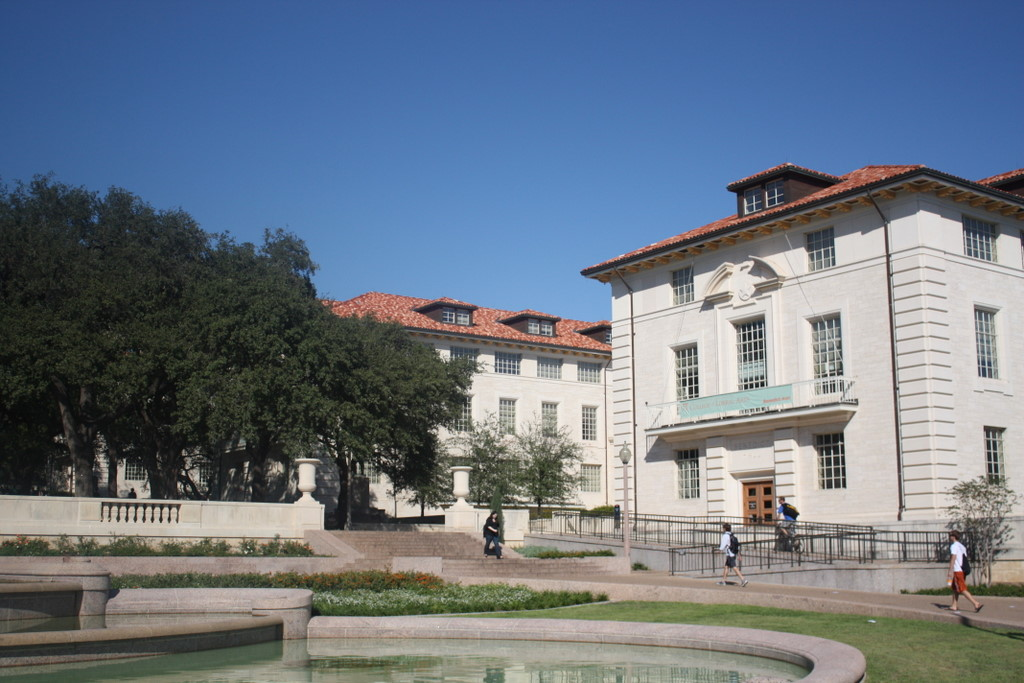
\includegraphics[width=7cm]{uttower1.jpg}
\end{minipage}
\begin{minipage}[t]{0.48\textwidth}
\centering
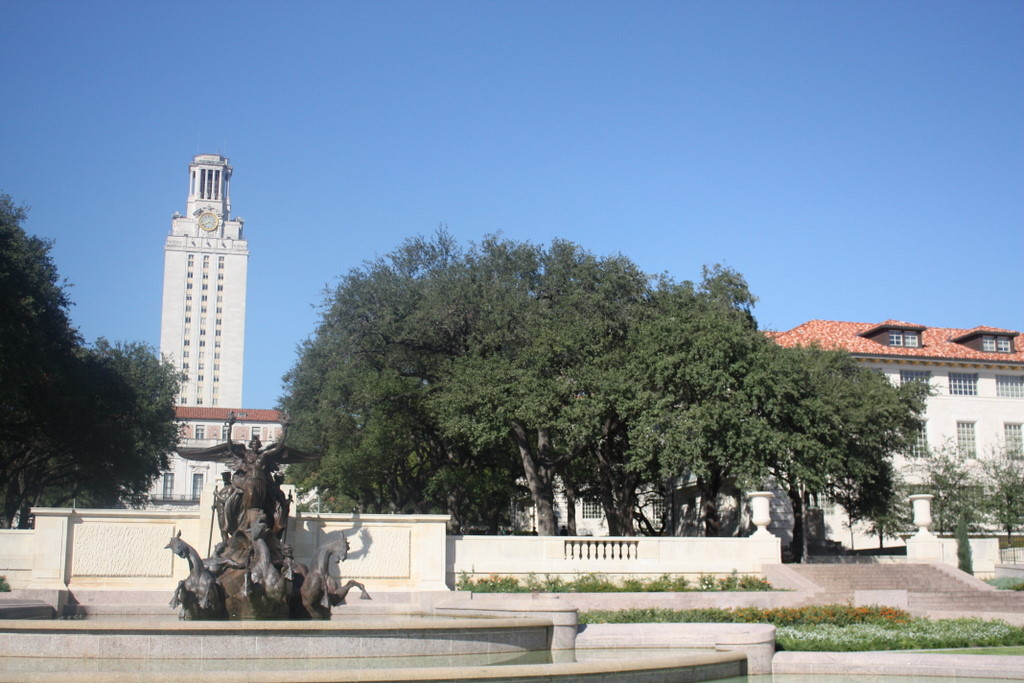
\includegraphics[width=7cm]{uttower2.jpg}
\end{minipage}
\end{figure}
\begin{figure}[h]
	\centering  %centering image
	\includegraphics[width=15cm]{Mosaicos_1.png}  % load image
\end{figure}

\newpage
\subsubsection{NJU pictures I took:}
Reproduce:
code.py: Choose $2$ (0 阶插值:450s;1 阶插值:3000s,默认0阶插值)
\begin{figure}[!h]
\centering
\begin{minipage}[t]{0.48\textwidth}
\centering
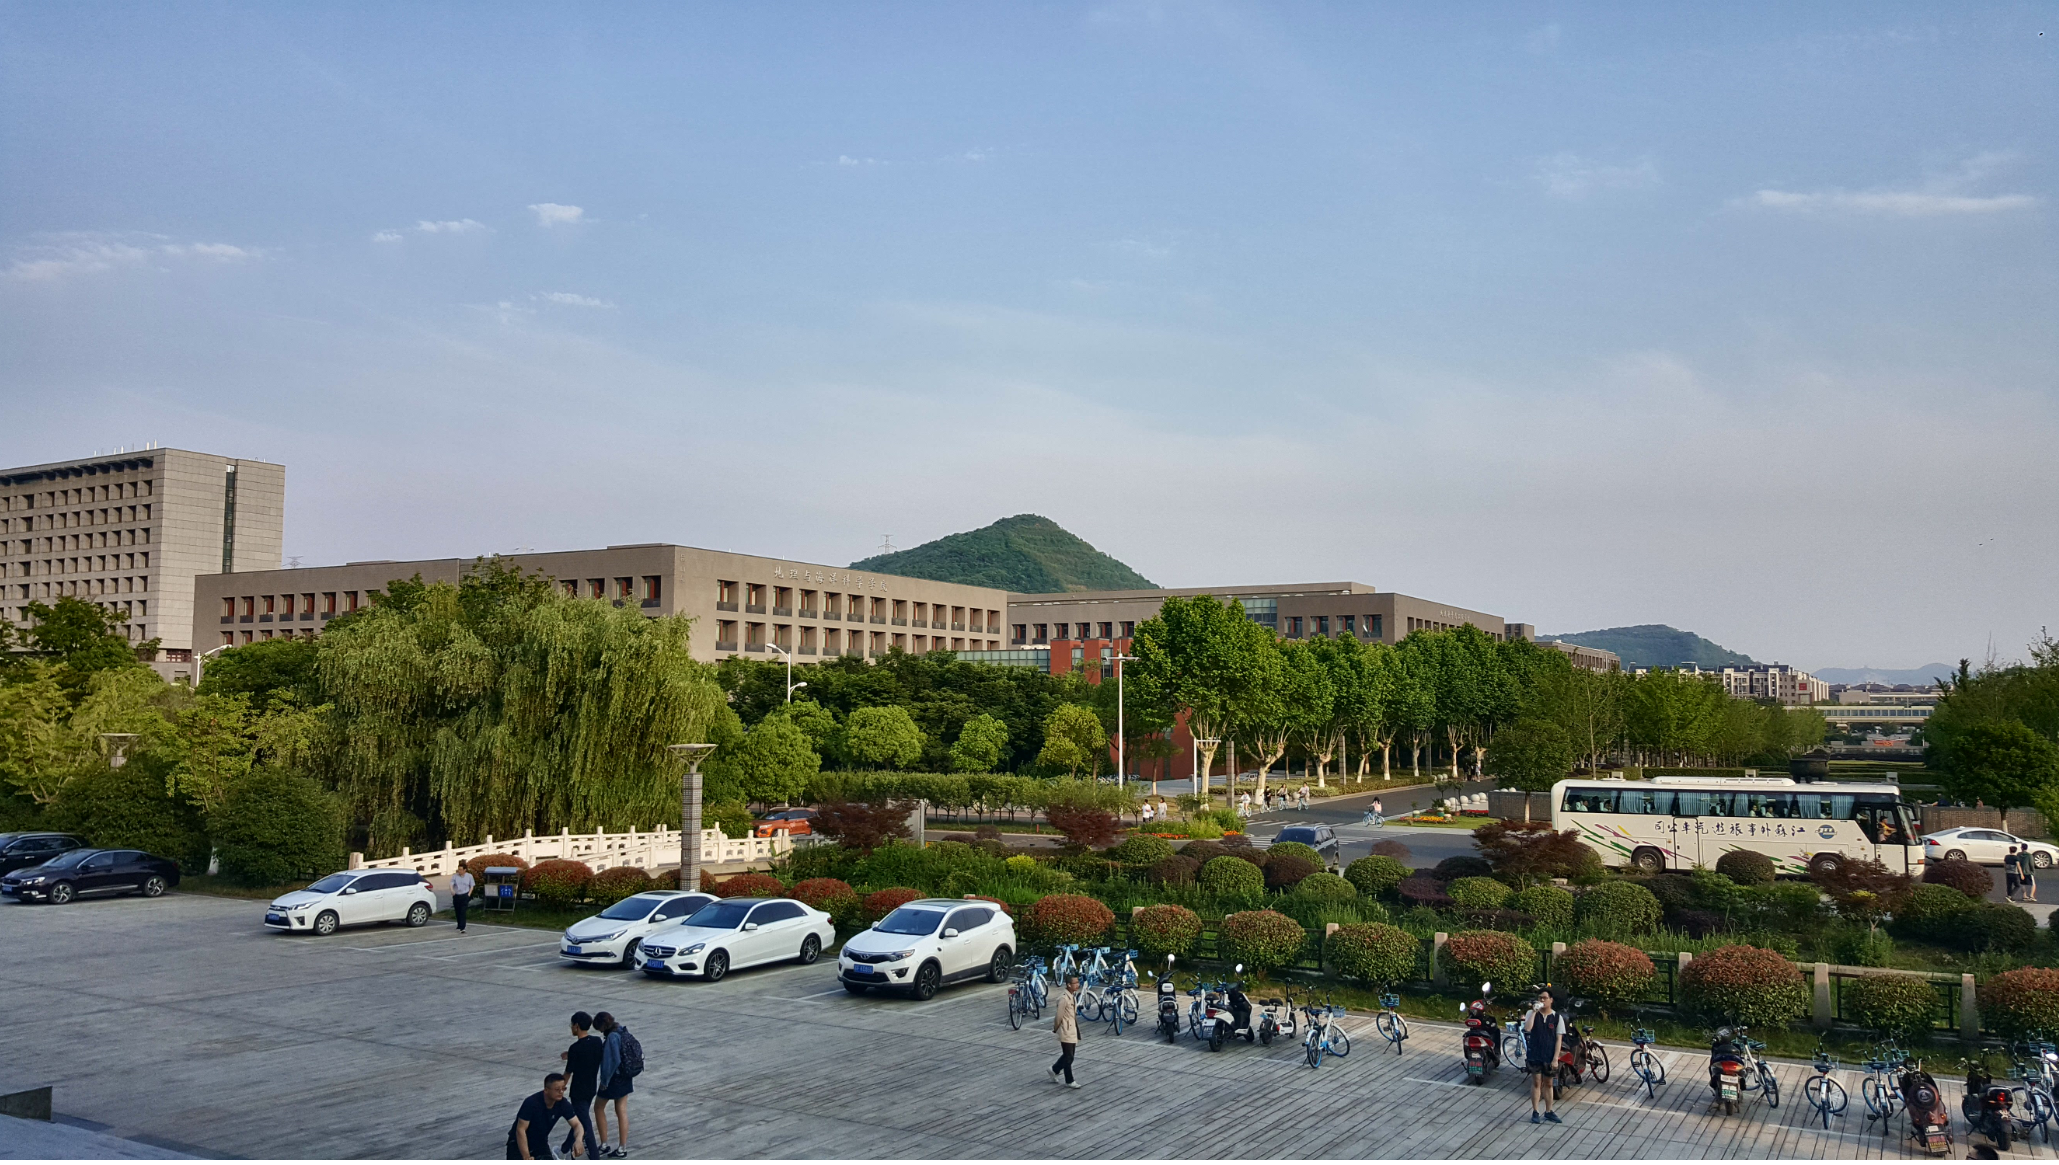
\includegraphics[width=7cm]{NJU1.png}
\end{minipage}
\begin{minipage}[t]{0.48\textwidth}
\centering
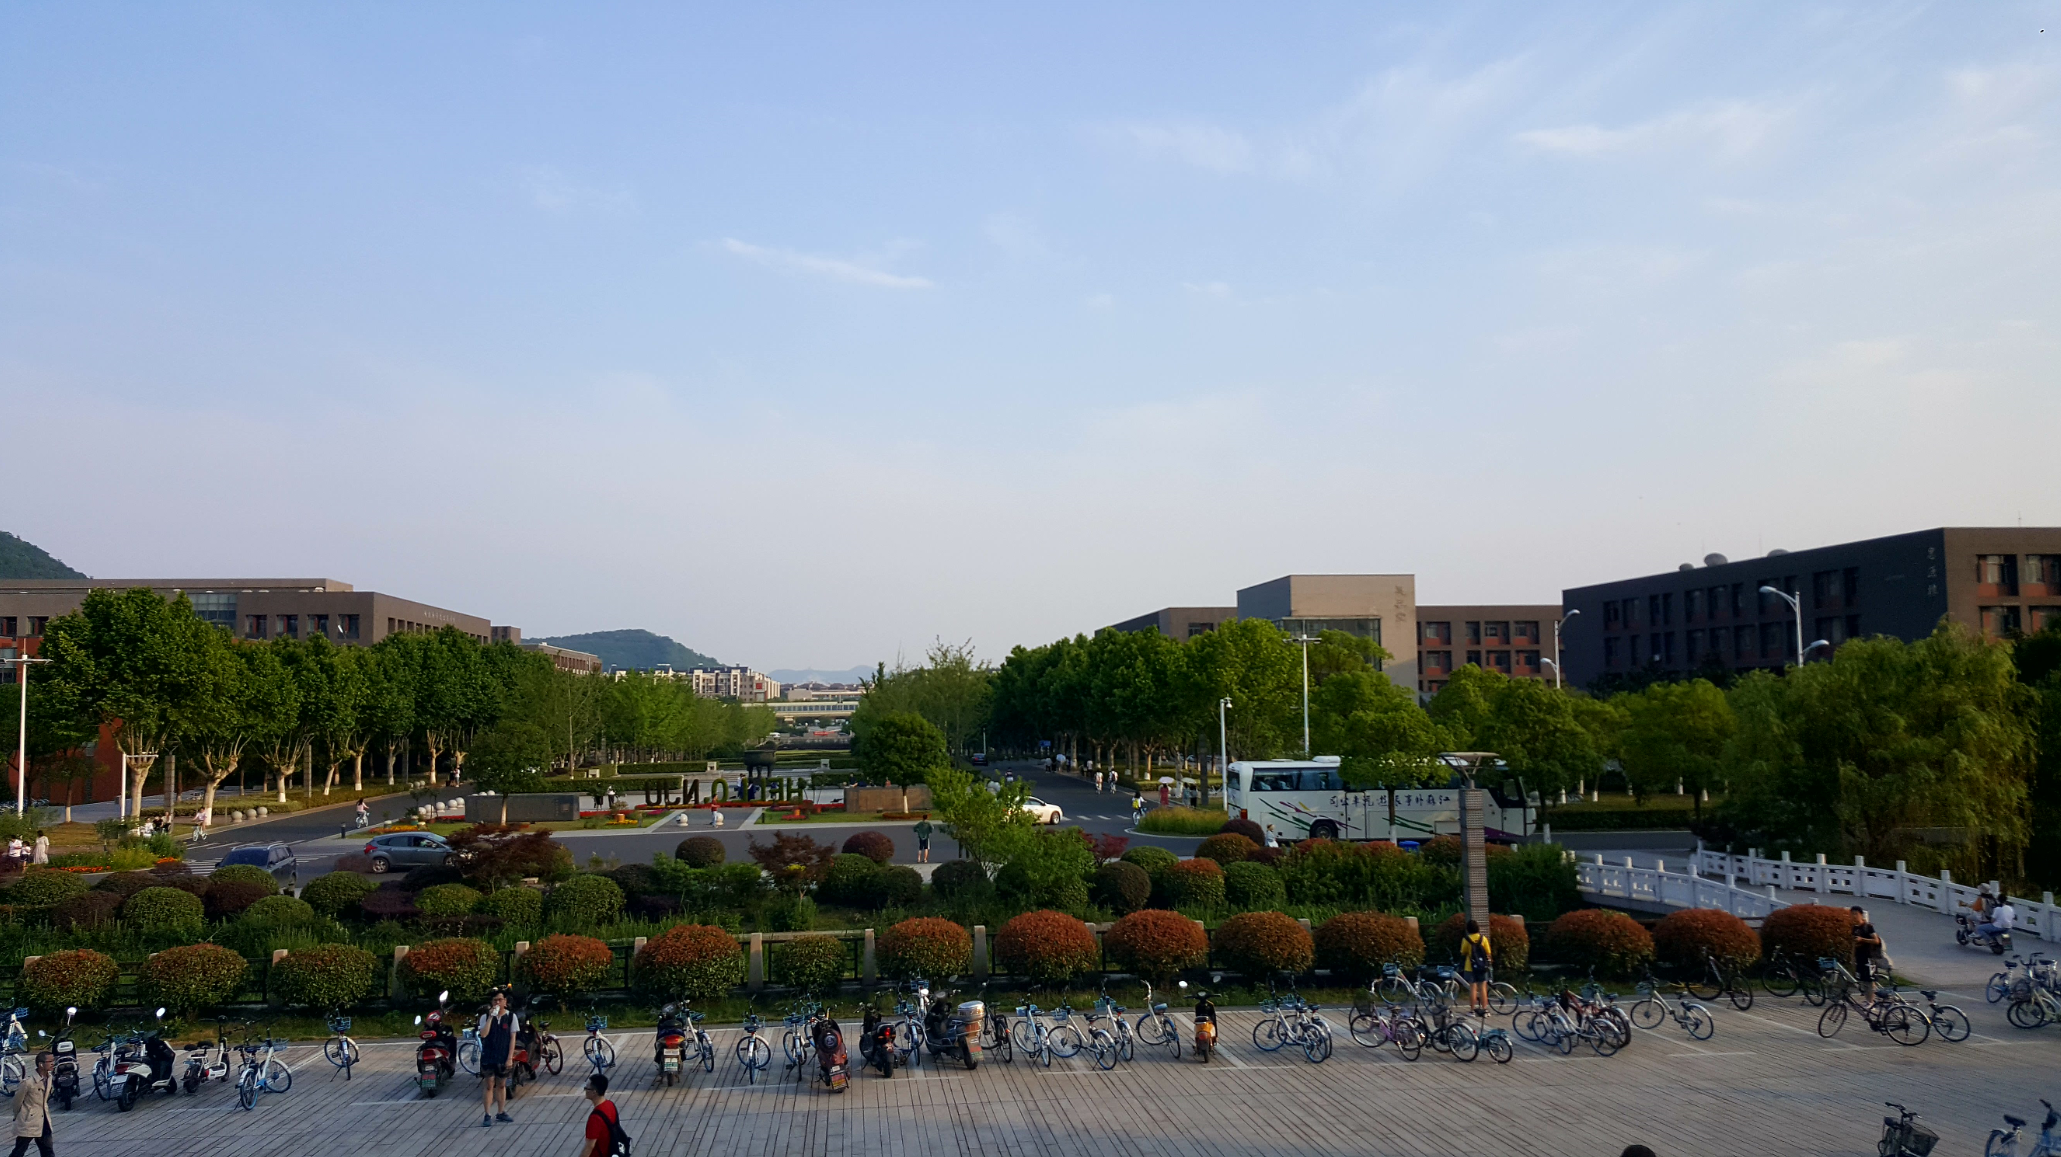
\includegraphics[width=7cm]{NJU2.png}
\end{minipage}
\end{figure}
\begin{figure}[th]
	\centering  %centering image
	\includegraphics[width=12cm]{NJU.png}  % load image
\end{figure}
\begin{figure}[th]
	\centering  %centering image
	\includegraphics[width=12cm]{NJU0.png}  % load image
\end{figure}

\newpage
\subsubsection{Tom and Jerry in billboard:}
Reproduce:
code.py: Choose $3$ (0 阶插值:20s;1 阶插值:90s,默认0阶插值)
\begin{figure}[!h]
\centering
\begin{minipage}[t]{0.48\textwidth}
\centering

\includegraphics[width=7cm]{test1-3-in.jpg}
\end{minipage}
\begin{minipage}[t]{0.48\textwidth}
\centering
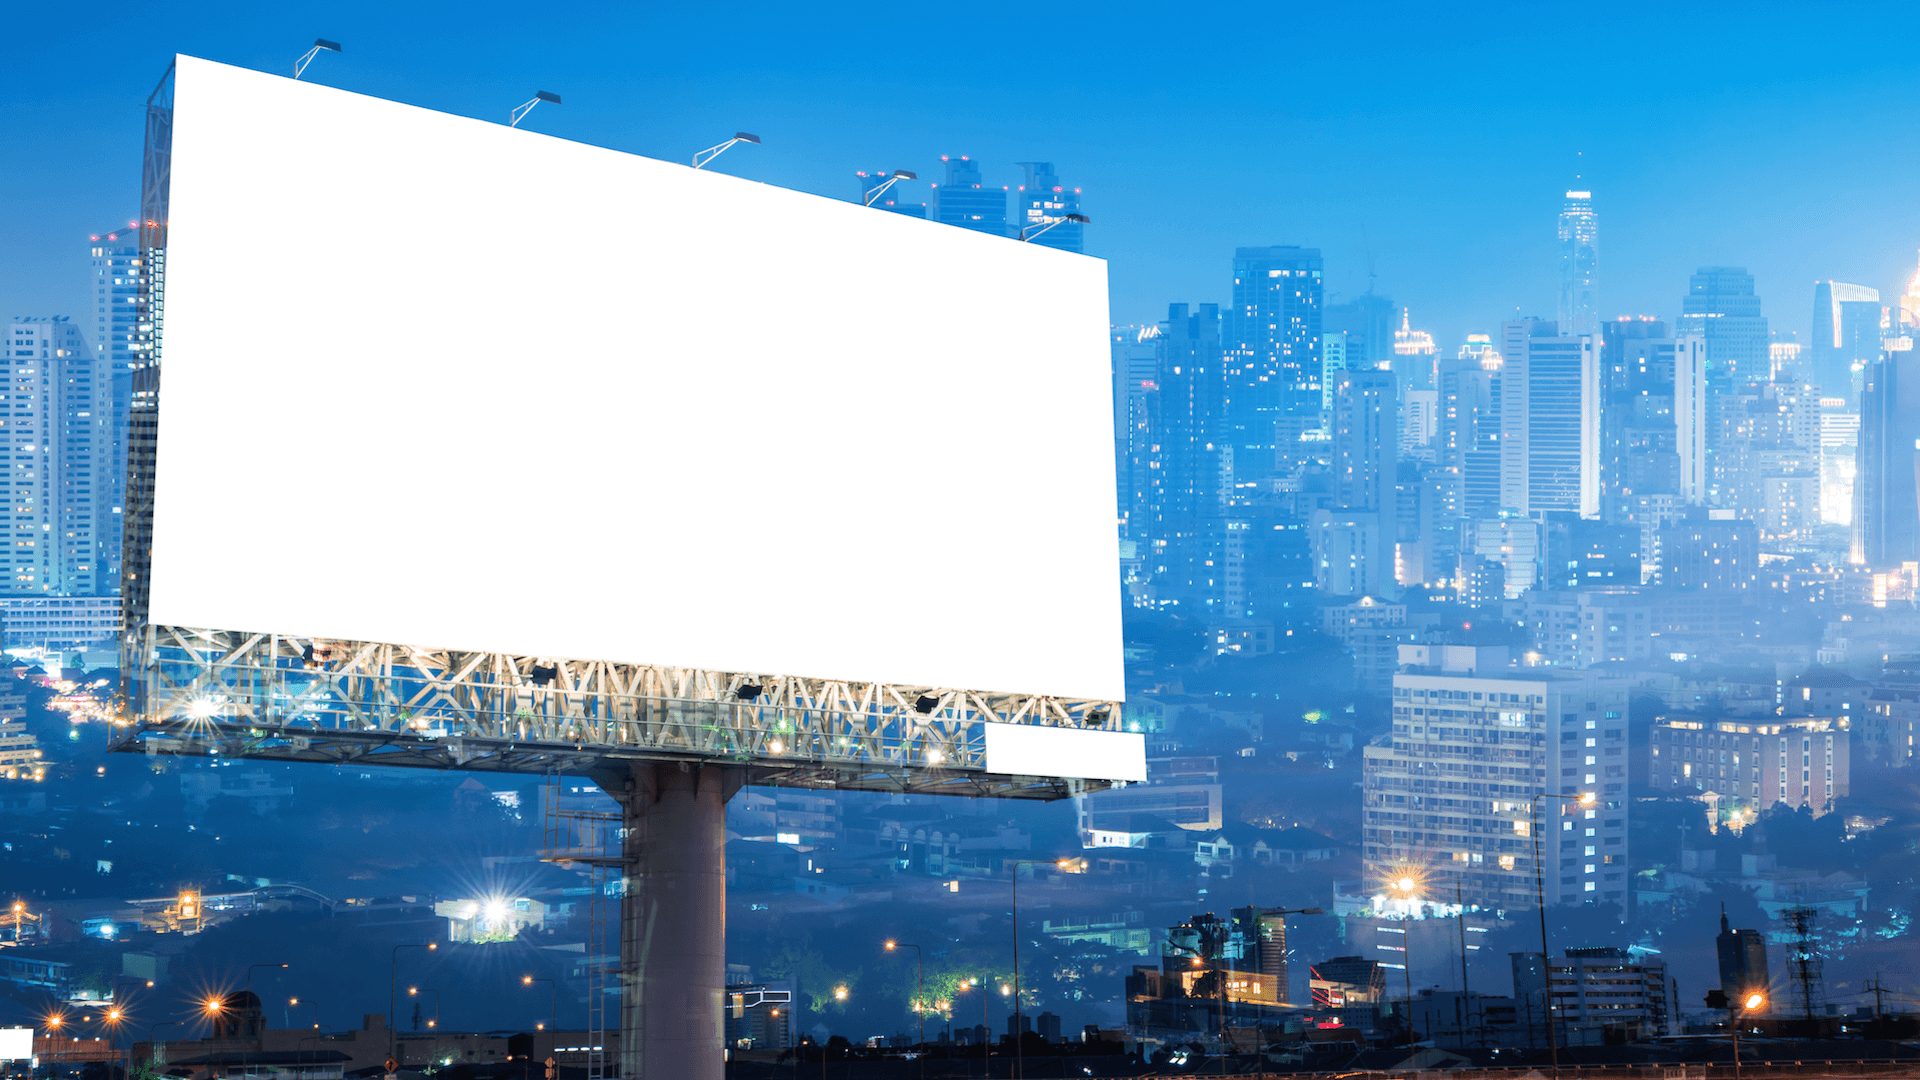
\includegraphics[width=7cm]{test1-3.png}
\end{minipage}
\end{figure}
\begin{figure}[h]
	\centering  %centering image
	\includegraphics[width=14cm]{Tom_board.png}  % load image
\end{figure}



\newpage
\section{Automatic Image Mosaics [20 pts]}
\subsection{SIFT [10 pts]}
\begin{figure}[!h]
\centering
\begin{minipage}[t]{0.48\textwidth}
\centering
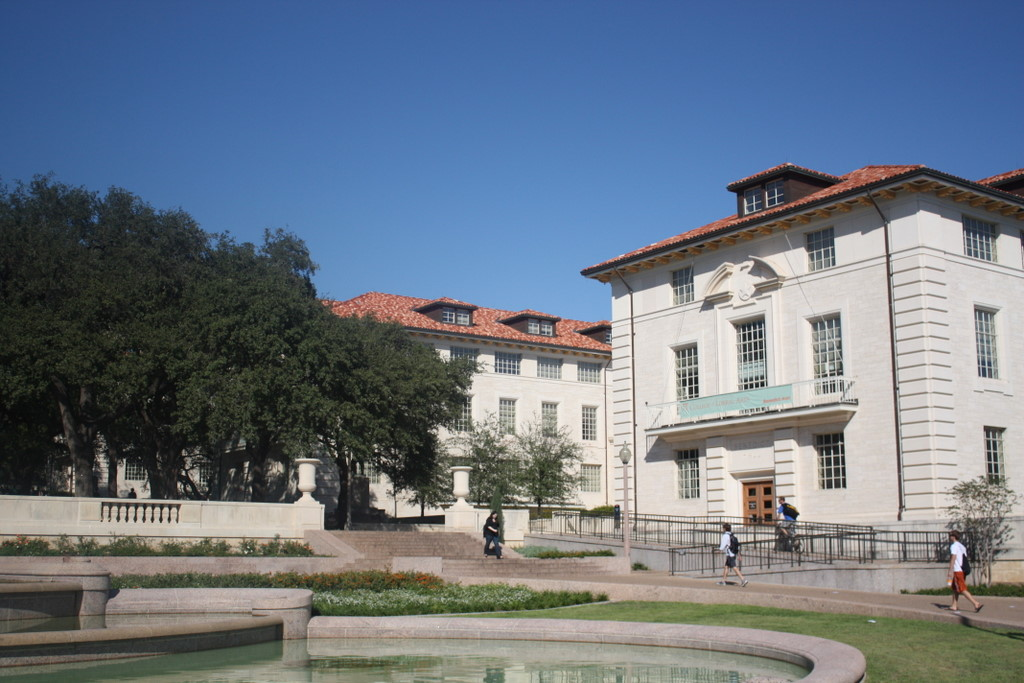
\includegraphics[width=7cm]{uttower1.jpg}
\end{minipage}
\begin{minipage}[t]{0.48\textwidth}
\centering
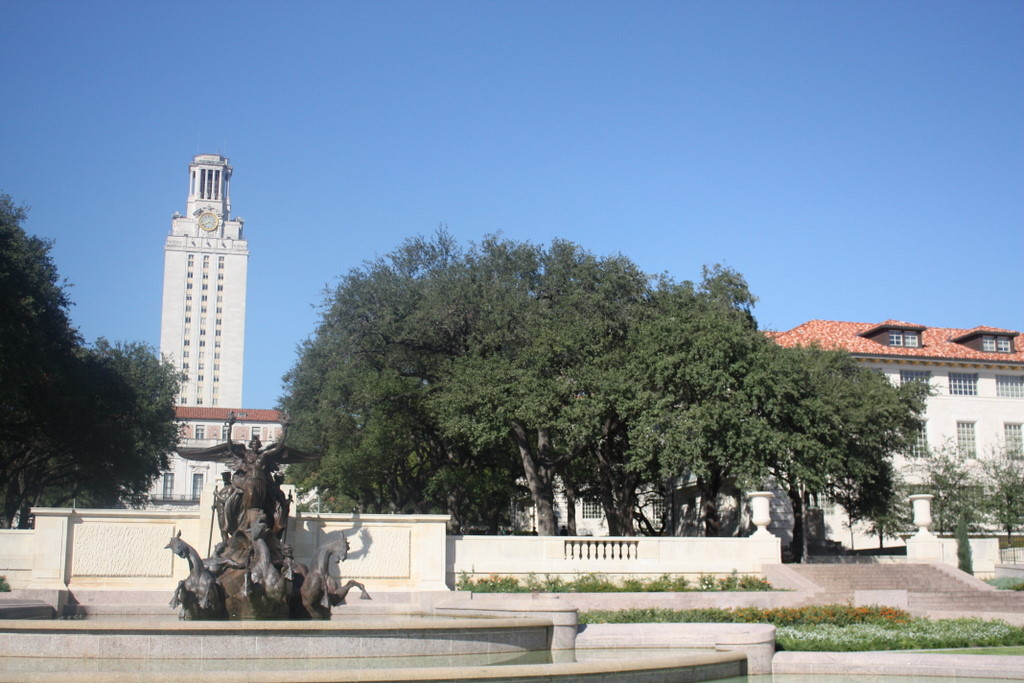
\includegraphics[width=7cm]{uttower2.jpg}
\end{minipage}
\end{figure}

\begin{figure}[h]
	\centering  %centering image
	\includegraphics[width=14cm]{uttower10.png}  % load image
	\caption{SIFT choose 10 best}
\end{figure}

\begin{figure}[h]
	\centering  %centering image
	\includegraphics[width=14cm]{uttower100.png}  % load image
	\caption{SIFT choose 100 best}
\end{figure}

\begin{figure}[h]
	\centering  %centering image
	\includegraphics[width=14cm]{uttower200.png}  % load image
	\caption{SIFT choose 200 best}
\end{figure}

\newpage

\newpage
\subsection{RANSAC [10 pts]}
\begin{figure}[h]
	\centering  %centering image
	\includegraphics[width=14cm]{uttower_SIFT100_RANSAC.png}  % load image
	\caption{SIFT choose 100 best with RANSAC}
\end{figure}
\begin{figure}[h]
	\centering  %centering image
	\includegraphics[width=14cm]{uttower_SIFTall_RANSAC.png}  % load image
	\caption{SIFT choose all with RANSAC}
\end{figure}


\end{document}